\section{bHash Design and Implementation}

\label{sec:bhash}


In this section, we present the design and implementation of bHash in detail. bHash needs two passes of the whole set of kv-pairs, so it is a two-phase algorithm. The first phase is statistics collection phase (see Figure \ref{fig:bHash}) and the second phase is file filling phase (see Figure \ref{fig:bHash}). Statistics collection phase studies the global knowledge of group size information and generates a pos\_table that contains $\langle group key, file position\rangle$s. File Filling phase writes out kv-pairs to certain file positions according to the offset\_table. To reduce the number of I/Os, we exploit an output buffer design in the second phase which converts a large number of small random writes to less number of big sequential writes. Furthermore, by partitioning the kv-pairs groups in the first phase and processing kv-pairs partition-by-partition in the second phase, we can constrain the key range in each partition and make the kv-pairs more concentrate on a few keys in each partition of groups. As result, more benefits from the buffer design can be gained, i.e., more efficient big sequential writes are produced. In the following, we describe the two phases in detail and provide a complexity analysis.

%to obtain the global data distribution knowledge, i.e., $\langle group key, group size\rangle$ information. bHash goes a step further to split the source file into sub files that the key range covered by every sub file does not overlap by using horizontally partitioning the hash table similarly to \cite{lejsek2009nv}, \cite{gedik2014partitioning} simultaneously. With the group size knowledge from first phase, Hash Grouping phase assumes the sorted file structure and compute every group's output position in the sorted file. Given the size information of every group, the output file position (offset) can be calculated by accumulating the group size. Then bHash will obtain an in-memory table contains $\langle groupkey,fileposition\rangle$ information. Finally, Hash Grouping phase needs another pass of the input file and outputs kv-pairs to file in terms of the previously obtained $\langle groupkey,fileposition\rangle$ information. Hash Grouping phase is applied independently in each sub file in a top-down fashion. The width of the sub file��s partition is adjusted dynamically based on how many file numbers the user has specified. This allows bHash to use only a small part of the source file for grouping at a time, rendering the algorithm cache-friendly and minimizing the disk I/O overhead. Each sub file represents an independent unit and groups among different sub files have no intersection, which can be guaranteed by horizontally partitioning hash buckets. For all kv-pairs mapped to a hash bucket, their positions in the hash bucket are consistent with the order of appearance. The source file is divided into multiple sub files, the key range covered by a sub file will be reduced by several multiples. Grouping a sub file at a time makes grouping results more closely. In the case of a fixed memory buffer size, the number of groups included in a sub file will be fewer so that more kv-pairs in one group will be cached in buffer. One seek operation can write more kv-pairs and the total number of seek will decrease obviously. To sum up, bHash benefits from both hash table��s random access ability (from hash-based grouping) and sorted structure��s sequential access ability (from sort-based grouping).

%The structure of this section is as follows. Section 3.1 describes the Group Size Accumulating phase and section 3.2 explains Hash Grouping phase. Section 3.3 discusses algorithm optimization and section 3.4 contains a discussion on time complexity.

\begin{figure}%figure 3
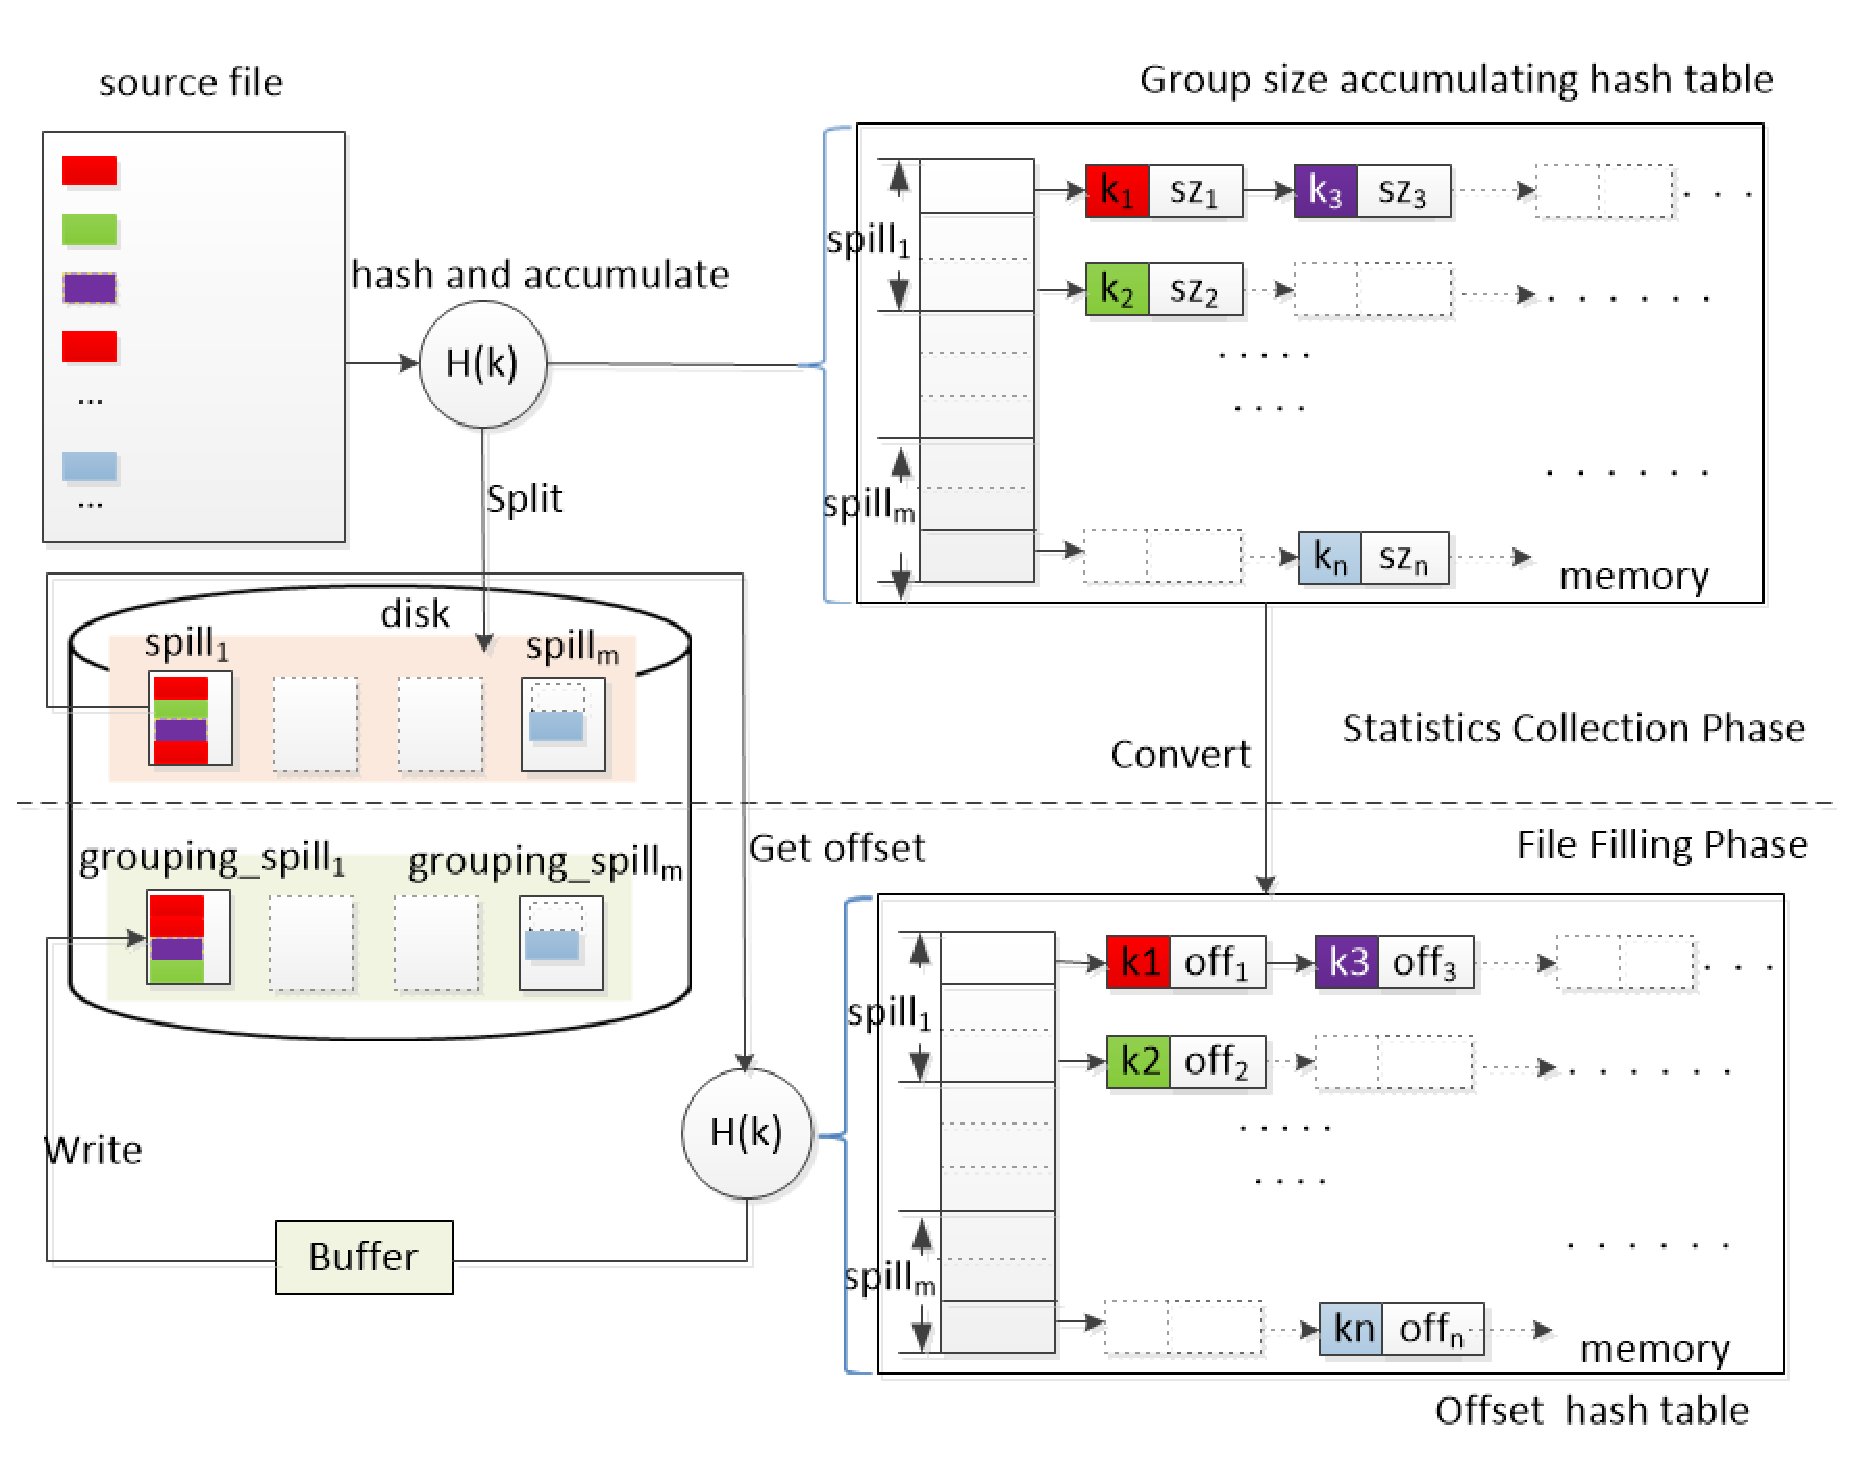
\includegraphics[width=.5\textwidth]{fig/bHash}
\caption{Overview Intuition of bHash.}
\label{fig:bHash}
\end{figure}

%\begin{figure}%figure 4
%\includegraphics[width=.5\textwidth]{Hashgroupingstage}
%\caption{Hash grouping phase.}
%\end{figure}

\subsection{Phase 1: Statistics Collection}%3.1

The first phase needs one pass of the whole input kv-pairs file and writes them out to multiple smaller files, which is referred to as \emph{spills}. In the first phase, multiple functions involved are described as follows.

%\Paragraph{Group Size Accumulation}

\textbf{Group Size Accumulation.} As shown in Figure \ref{fig:bHash}, an in-memory hash table is maintained to accumulate the value size for each key. The size of values indexed by the same key is accumulated in the value size table. By one pass of the whole set of input kv-pairs contained in source file we will obtain the value size table indexed by keys. Note that, the number of hash buckets $b$ in the group size table balances the memory cost and the query time cost, which will be discussed in Section \ref{sec:param}.


%\Paragraph{Kv-Pairs Reorganization}

\textbf{KV-Pairs Reorganization.} Recall that there is an output buffer (in the file filling phase) which aims at merging a large number of small random writes to less number of big sequential writes. If the random output kv-pairs are more concentrate on a key range, they are more likely to be continuously written out. That is, they can be merged together as less number of big sequential write. To improve the output buffer efficiency in the file filling phase, we should reorganize the read-in kv-pairs in a smart way.

Our idea is to partition the kv-pairs and assign the kv-pairs that are in the same partition with close write-out positions, such that the partition-by-partition processing of kv-pairs in file filling phase is likely to result in big sequential writes. Specifically, we partition the kv-pairs into multiple \emph{partitions}. This can be achieved by hashing, i.e., multiple $\langle key, value group \rangle$s sharing the same $H_g(key)$ are grouped together, where $H_g()$ is a hash function. The keys in the same partition are assigned with close write-out positions. These kv-pairs in the same partition are written out in a \emph{spill} as shown in Figure \ref{fig:bHash}. Note that, the recorded write-out position is not for the spill but for the final output file (i.e., grouping\_spill in Figure 2) with grouped kv-pairs.

%\Paragraph{Offset\_Table Generation}
\textbf{Offset\_Table Generation.} We then convert the value-size table to offset\_table. Given the size of each key and the size of values for each key, we can calculate how many bytes a $\langle key, value group\rangle$ pair will take up in the final output file. With a specific output order, we can calculate the write-out position (i.e., offset) for each $\langle key, value group\rangle$. As mentioned above, the output order should be determined according to the partition information. The $\langle key, value group \rangle$s in a partition are written out in a continuous order, so that these keys are assigned with continuous write-out positions. This can be done by incrementally assigning write-out positions partition-by-partition and within each partition.

%Let \emph{F} be the source file to be aggregated and \emph{T} be the group size accumulating hash table that each entry corresponds to a group. The phase mainly completes sub file division and group size accumulating. Let \emph{S} be the set of final grouping files and the dimension of \emph{S} is initialized by the sub file number \emph{m} specified by users. At the beginning, a empty hash table \emph{T} will be created, the basic array��s size has been set to \emph{b}, i.e., the number of hash buckets in table \emph{T}. If the number of hash buckets \emph{b} is too small, kv pairs mapped into one bucket will become a few more. The time of finding an entry in a hash table is proportional to the length of the bucket the record mapped to. However, too many hash buckets will require more memory, so the number of buckets \emph{b} must be an appropriate value to balance time cost and memory cost. Related parameters setting are given in section 4.

%$p_1^{t_1}$ $S=\{{p^{t_i}_i}\}^N_{i=1}$}

%It means that the hash table is partitioned horizontally into \emph{m} parts from top to down. The kv pairs mapped to the first $b/m$ buckets will be stored in sub file $file_0$ and mapped to the last $b/m$ buckets will be stored in sub file $file_{m-1}$ . After all the data in the source file has been processed, we can obtain the size of each group and kv pairs in the source file have been partitioned into several sub files. Each sub file represents an independent unit and groups among different sub files have no intersection, the key range covered by a sub file will be reduced by several multiples, which reduces the number of seek in the subsequent hash grouping phase.

\subsection{Phase 2: File Filling}%3.2

The offset\_table stores the output file position (i.e., offset) for each $\langle key, value group \rangle$. Given this deterministic information, the second phase runs as a file filling process by taking the spills as input. It reads in and processes the spills one by one. Referring to the in-memory offset\_table, the kv-pairs in spills are written out to specific positions in the final output file.

The profiling of this process shows that large amount of time is spent on seek operations during the file filling. This is mainly due to the fact that the writing of kv-pairs is not necessarily sequential. Recall that in the first phase the kv-pairs has been split into multiple partitions (i.e., spills) and their write-out positions have been reorganized from partition to partition. By processing each partition (spill) at a time, we can narrow the range of seek operations so as to reduce the seek distance (seek time).

%\Paragraph{Reordering KV-Pairs in Output Buffer}

\textbf{Reordering KV-Pairs in Output Buffer.} We have an output buffer design as shown in Fig 2. which buffers the write-out kv-pairs and reorders them according to their positions (i.e., offsets) before writing them out. It will 1) merge a large number of random small writes to less number of sequential big writes and 2) avoid frequent backward-and-forward disk arm movement. The ideal buffer size is equal to the size of an input spill, so that the buffer can hold all the kv-pairs in that spill. By using any $O(1)$ space requirement sorting algorithm (e.g., quick sort), we can sort these kv-pairs in terms of their offsets and output them with only one single sequential write without any random write operations.


%Without any extra reordering, we buffer these kv-pairs in their group entry of the offset table. Flushing the buffer only requires to traverse partial hash buckets that belong to the spill sequentially.
The spill size somehow depends on how the hash partition in the first phase is defined. We can set the hash partition function to generate more or less partitions to obtain smaller or bigger spills. However, the sizes of spills might be greatly different from each other due to the skewed data distribution. We cannot build a fix-sized buffer by assuming equal-sized spills. It is also possible that the memory budget is not enough to create the buffer when a certain spill is extremely large. A simple design is to buffer as many kv-pairs as possible and dump them together. Without any extra sorting, we buffer these kv-pairs in their group entries of the offset table. Flushing the buffer only requires to traverse partial hash buckets that belong to the spill sequentially. Because the offset of each group is calculated based on the previous entry, the offset for each group saved in hash entry is incremented sequentially bucket-by-bucket and within each bucket. In this way, seek operations of different groups will be in order, it allows us to flush the buffer by scanning sequentially the output file (i.e.,grouping\_spill). Note that, even though a random seek is performed, the seek time is expected to be very small because the next offset is physically very close to the current disk head position. The experiment shows that the gain is up to 10\%.
% Alternatively, we can borrow the idea from online live streaming which has a receive buffer for reordering the video packets \cite{}. It renders the video frames immediately as long as necessary packets have been received and at the same time releases the buffer space for future incoming packets. In our case, we have the similar requirements for the buffer design and can utilize XXX technique \cite{} to improve the buffer efficiency.

%\Paragraph{I/O Benefit Analysis}
\textbf{I/O Benefit Analysis.} In the following, we formally analyze the benefit of our \emph{partition-and-buffer} design that includes the $\langle key, value group \rangle$s partitioning in the first phase and the reordering buffer in the second phase. As known, the amount of I/O is the same no matter with or without the partition-and-buffer design. We focus on analyzing the seek distance, which plays a key role to I/O performance. We pose the following theorem to demonstrate the gained I/O benefit.

\begin{theorem}\label{theo:iobenefit}
Suppose without partitioning in the first phase, i.e., only one spill is produced after the first phase, with a fixed buffer size, it is required an expected total seek distance $D$ to generate the kv-pairs grouped output file. If we utilize partitioning and have $m$ spills, with the same buffer size, the expected total seek distance is $\frac{D}{m^2}$.
\end{theorem}
\begin{proof}
(1) Without partitioning. By using the buffer that reorders the kv-pairs in terms of their offsets, we can guarantee that the file filling after each buffer dumping never goes backward and forward. Suppose a buffer reorders $k$ unique keys with their values, and the average seek distance for writing each kv-pair is $d$. The total expected seek distance after each buffer dumping is $k\cdot d=D_b$.

(2) With partitioning. Since partitioning narrows the scope of key range by $\frac{1}{m}$, the average seek distance for writing each kv-pair is $\frac{d}{m}$. Furthermore, by partitioning the number of unique keys in buffer is also reduced to $\frac{k}{m}$ on average. The total expected seek distance after each buffer dumping is $\frac{k\cdot d}{m^2}=\frac{D_b}{m^2}$.

Since the amount of data is the same, the number of buffer dumping is the same for the above two cases, i.e., $\sum{D_b}=D$. Therefore, if there is total $D$ seek distance without partitioning, we only need $\frac{D}{m^2}$ seek distance with partitioning.
\end{proof}
%\subsection{Parallel Execution}
%phase 1: multiple I/O threads for spilling on SSD.
%phase 2: multiple processing threads and I/O threads for reordering every spill
%
%\textcolor{red}{this part is necessary for the completeness and can add credit. whether to implement it or not is up to you.}
\begin{algorithm}[ht]
    \caption{bHash}
  \label{tab:group}
    \begin{algorithmic}[1]
\Require  File \emph{F} , sub file number \emph{m} , hash buckets number \emph{b}
    \Ensure set of result files $R$
     \State \emph group size accumulating hash table \emph{T:=} a basic array of size \emph{b}
       \State \emph{S:=}\{\textbf{for} each \emph{i} \textbf{do} generate a file $spill_i$, \emph{0 $\textless$ i $\le$m}\}
         \State \emph{R:=}\{\textbf{for} each \emph{i} \textbf{do} generate a file $grouping\_spill_i$, \emph{0 $\textless$ i $\le$ m}\}
     \For{ each input $\langle key,value\rangle$ in \emph{F}}
      \State calculate the hash value H(key) on key
     \State check for a matching row in the hash table
     \If {there is no match}
     \State insert a entry (key,sizeof($\langle key,value\rangle$)) into \emph{T}
     \Else
     \State update the matching entry's group size with the sizeof($\langle key,value\rangle$)
     \EndIf
     \State $id=H(key)\%(b/m)$
     \State append the $\langle key,value\rangle$ to the partition file  $spill_{id}$
     \EndFor
     \State offset hash table $O:=Convert(T)$
     \For{ each $spill_i \in S$ ,\emph{0 $\textless$ i $\le$ m}}
     \For{ each input $\langle key,value\rangle$ in $spill_i$}
      \State calculate the hash value \emph{H(key)} on key
      \State $id=H(key)\%(b/m)$
     \State check for a matching key and get the $off_{key}$ of key from $O$
     \State write the $\langle key,value\rangle$ to the $off^{th}_{key}$ bytes of the file $grouping\_spill_i$
      \State the matching entry's offset is increased by sizeof($\langle key,value\rangle$)
     \EndFor
     \State remove the $spill_i$ from $S$
     \EndFor
    \State output \emph{R}
    \end{algorithmic}
\end{algorithm}
\subsection{Making Them Together}

We summarize the whole process including the first phase and second phase in Algorithm 1. The algorithm starts by creating a working set containing \emph{m} sub files. Then the entire input file \emph{F} is scanned to calculate the size of each group in the working set. For a kv pair, calculate the hash value $H_{key}$ , then check whether there is a matching grouping entry in the hash table. If there is no a matching entry whose key is equal to the current key, insert a new entry that the first key is the current key and the second group size is the size of current kv-pair in bytes. If there is a matching group already, update the matching entry's group size like Formula 1.
\begin{equation}\label{eq:freshness}
    f_{key} += sizeof(key)+sizeof(value).
\end{equation}
\par{The next step is to output the current kv-pair to sub file, the id of corresponding file can be obtained from Formula 2.}
\begin{equation}\label{eq:freshness}
    id = H(key)\%(b/m).
\end{equation}
It means that the hash table is partitioned horizontally into \emph{m} parts from top to down. The kv-pairs mapped to the first $b/m$ buckets will be stored in sub file $spill_1$ and mapped to the last $b/m$ buckets will be stored in sub file $spill_m$ . After all the data in the source file have been processed, we can obtain the size of each group and kv-pairs in the source file have been partitioned into several sub files(as shown 4-14 in algorithm 1).

Before the file filling phase really begins, we need to convert every group size to the file position information (i.e.,offset, see line 15 in Algorithm 1). The $Convert$ function traverses the group size accumulating hash table $T$, in more details, traverses hash buckets in the same partition from top to down and from left to right for a bucket. The first entry of the first bucket in the $i^{th}$ partition is the first group of the $i^{th}$ partition, so the initial offset of the entry equals to 0. The initial offset of an entry means that the first kv-pair mapped to the group will be stored in the ${(initial \; offset)}^{th}$ bytes of the grouping sub file $grouping\_spill_i$. Define the group size of the previous entry as $f_{pre}$, which means that the size of the previous group is $f_{pre}$. Define the initial offset of the previous group as ${off}_{pre}$. So the offset of current entry ${off}_{cur}$ equals to the sum of ${off}_{pre}$ and $f_{pre}$. After calculate the offset of each group, bHash will obtain an in-memory table which contains $\langle groupkey,fileposition\rangle$ information. Finally, File Filling phase needs another pass of the spilting file and outputs kv-pairs to file in terms of the previously obtained $\langle groupkey,fileposition\rangle$ information(see lines 16-25 in Algorithm 1). Each sub file $spill_i$ is a processing unit. The entire input split is scanned sequentially as shown in Figure 2. For a kv-pair, calculate the hash value $H_{key}$ and get the offset ${off}_{key}$  by searching the hash bucket $H_{key}$. Then, the kv-pair will be wrote to the ${off}^{th}_{key}$ bytes of the result file $grouping\_spill_{id}$. With a kv-pair from sub file $spill_{i}$ having been output, the current offset of the corresponding group will increase the size of the kv-pair in bytes, which indicates the next kv-pair mapped to the same group will be stored in the ${({off}_{cur} + sizeof(\langle key,value\rangle ))}^{th}$ bytes of the grouping sub file $spill_{id}$(line 22 in Algorithm 1). Specifically, some buffer optimizations have been applied as shown in section B. Grouping a sub file at a time, the key range is covered in a sub file, so the seek operation only appears in one file, which is the main reason of splitting.

To sum up, bHash benefits from both hash table��s random access ability (from hash-based grouping) and sorted structure��s sequential access ability (from sort-based grouping).

%\begin{algorithm}[ht]
%    \caption{Hash Grouping}
%  \label{tab:commands}
%    \begin{algorithmic}[1]
%\Require  set of sub files $S$, group size accumulating hash table $T$, sub file number $m$, hash buckets number $b$
%    \Ensure set of result files $R$
%     \State \emph{R:=}\{\textbf{for} each \emph{i} \textbf{do} generate a file $file_i$, \emph{0 $\le$ i $\textless$ m}\}
%       \State offset hash table $O:=Convert(T)$
%     \For{ each $file_i \in S$ ,\emph{0 $\le$ i $\textless$ m}}
%     \For{ each input $\langle key,value\rangle$ in $file_i$}
%      \State calculate the hash value H(key) on key
%      \State $id=H(key)\%(b/m)$
%     \State check for a matching key and get the $off_{key}$ of key from $O$
%     \State write the $\langle key,value\rangle$ to the $off^{th}_{key}$ bytes of the file $file_{id}$
%      \State the matching entry's offset is increased by sizeof($\langle key,value\rangle$)
%     \EndFor
%     \State remove the $file_i$ from $S$
%     \EndFor
%    \State output \emph{R}
%    \end{algorithmic}
%\end{algorithm}

\begin{comment}
The algorithm starts by creating a working set containing \emph{m} sub files (see Figure 3). Then the entire input file \emph{F} is scanned to calculate the size of each group in the working set. For a kv pair, calculate the hash value $H_{key}$ , then check whether there is a matching grouping entry in the hash table. If there is no a matching entry whose key is equal to the current key, insert a new entry that the first key is the current key and the second value size is the size of current kv pair in bytes. If there is a matching group already, update the matching entry's value size like Formula 1.
\begin{equation}\label{eq:freshness}
    f_{key} += sizeof(key)+sizeof(value).
\end{equation}
\par{The next step is to output the current kv pair to sub file, the id of corresponding file can be get from Formula 2.}
\begin{equation}\label{eq:freshness}
    id = H(key)\%(b/m).
\end{equation}


\begin{algorithm}[ht]
    \caption{Group Size Accumulating}
  \label{alg:group}
    \begin{algorithmic}[1]
\Require  File \emph{F} , sub file number \emph{m} , hash buckets number \emph{b}
    \Ensure set of sub files \emph{S}, group size accumulating hash table \emph{T}
     \State \emph{T:=} a basic array of size \emph{b}
       \State \emph{S:=}\{\textbf{for} each \emph{i} \textbf{do} generate a file $file_i$, \emph{0 $\le$ i $\textless$ m}\}
     \For{ each input $\langle key,value\rangle$ in \emph{F}}
      \State calculate the hash value H(key) on key
     \State check for a matching row in the hash table
     \If {there is no match}
     \State insert a new entry  [key,sizeof($\langle key,value\rangle$)] into \emph{T}
     \Else
     \State update the matching entry's value size with the sizeof($\langle key,value\rangle$)
     \EndIf
     \State $id=H(key)\%(b/m)$
     \State append the $\langle key,value\rangle$ to the partition file  $file_{id}$ in \emph{S}
     \EndFor
    \State output \emph{S}
    \end{algorithmic}
\end{algorithm}

It means that the hash table is partitioned horizontally into \emph{m} parts from top to down. The kv pairs mapped to the first $b/m$ buckets will be stored in sub file $file_0$ and mapped to the last $b/m$ buckets will be stored in sub file $file_{m-1}$ . After all the data in the source file has been processed, we can obtain the size of each group and kv pairs in the source file have been partitioned into several sub files. Each sub file represents an independent unit and groups among different sub files have no intersection, the key range covered by a sub file will be reduced by several multiples, which reduces the number of seek in the subsequent hash grouping phase.

During this phase, bHash constructs the grouping sub file for each sub file $file_i$. In Group Size Accumulating phase, the size of all groups has been accumulated in hash table. Before the hash grouping phase really begins, we need to convert every group size to the file position information (offset) of the group (line 2 in Algorithm 2). The $Convert$ function traverses the group size accumulating hash table $T$, in more details, traverses hash buckets in the same partition from top to down and from left to right for a bucket. The first entry of the first bucket in the $i^{th}$ partition is the first group of the $i^{th}$ partition, so the initial offset of the entry equals to 0. The initial offset of an entry means that the first kv-pair mapped to the group will be stored in the ${(initial \; offset)}^{th}$ bytes of the grouping sub file $file_i$. Define the group size of the previous entry as $f_{pre}$, which means that the size of data contained by the previous group is $f_{pre}$. Define the initial offset of the previous group as ${off}_{pre}$. So the offset of current entry ${off}_{cur}$ equals to the sum of ${off}_{pre}$ and $f_{pre}$. After calculate the offset of each group, bHash will obtain an in-memory table which contains $\langle groupkey,fileposition\rangle$ information. Finally, Hash Grouping phase needs another pass of the input file and outputs kv-pairs to file in terms of the previously obtained $\langle groupkey,fileposition\rangle$ information(see lines 3-12 in Algorithm 2). Each sub file $file_i$ is a processing unit. The entire input sub file is scanned sequentially as shown in Figure 4. For a kv-pair, calculate the hash value $H_{key}$ and get the offset ${off}_{key}$  by searching the hash bucket $H_{key}$. After getting the offset, the kv-pair will be wrote to the ${off}^{th}_{key}$ bytes of the result file $file_{id}$. With a kv-pair from sub file $file_{i}$ having been output, the current offset of the corresponding group will increase the size of the kv-pair in bytes, which indicates the next kv-pair mapped to the same group will be stored in the ${({off}_{cur} + sizeof(\langle key,value\rangle ))}^{th}$ bytes of the grouping sub file $file_{id}$(line 8 in Algorithm 2). Grouping a sub file at a time, the key range is covered in a sub file, so the seek operation only appears in one file, which is the main reason of splitting.


Contrary to previous key value grouping approaches, bHash provides us a method to build the grouping file without sorting. This is achieved using group size accumulating and hash grouping. In more detail, group size accumulating creates a group size hash table to record the size of different groups in bytes and splits the source file into several sub file in order to narrow the key range dealt with at a time. Then, Hash Grouping phase assumes the sorted file structure and computes every group's output position in the sorted file and do not really sort actually but only guarantee the kv-pairs in the same group to be locate together. To sum up, bHash benefits from both hash table��s random access ability (from hash-based grouping) and sorted structure��s sequential access ability (from sort-based grouping).
\begin{algorithm}[ht]
    \caption{Hash Grouping}
  \label{tab:commands}
    \begin{algorithmic}[1]
\Require  set of sub files $S$, group size accumulating hash table $T$, sub file number $m$, hash buckets number $b$
    \Ensure set of result files $R$
     \State \emph{R:=}\{\textbf{for} each \emph{i} \textbf{do} generate a file $file_i$, \emph{0 $\le$ i $\textless$ m}\}
       \State offset hash table $O:=Convert(T)$
     \For{ each $file_i \in S$ ,\emph{0 $\le$ i $\textless$ m}}
     \For{ each input $\langle key,value\rangle$ in $file_i$}
      \State calculate the hash value H(key) on key
      \State $id=H(key)\%(b/m)$
     \State check for a matching key and get the $off_{key}$ of key from $O$
     \State write the $\langle key,value\rangle$ to the $off^{th}_{key}$ bytes of the file $file_{id}$
      \State the matching entry's offset is increased by sizeof($\langle key,value\rangle$)
     \EndFor
     \State remove the $file_i$ from $S$
     \EndFor
    \State output \emph{R}
    \end{algorithmic}
\end{algorithm}


\subsection{Optimizing Disk Access}
The experimental evaluation and profiling of the Algorithm Hash Grouping shows that a significant amount of time is spent on seeking the result file. This is mainly due to the fact that the grouping process requires disk accesses that may not be sequential. Note that splitting has eliminated the seek operation among multiple files, which narrows the scope of disk head movement. As the Algorithm 2 shows that the algorithm groups a sub file at a time, we buffer partial grouping results in memory (see Figure 4) in order to write more kv-pairs per seek operation. If the buffer is full, these buffered partial grouping data will be flushed to the disk. Although partial grouping data of the same group has been buffered together and just need one seek operation, the seek operations of different groups may be out of order because kv-pairs from a sub file are out of order. To address this issue, we propose a novel buffer approach formed by modifying the entry structure of the group size accumulating hash table, as depicted in Figure 5.

\begin{figure}%figure 5
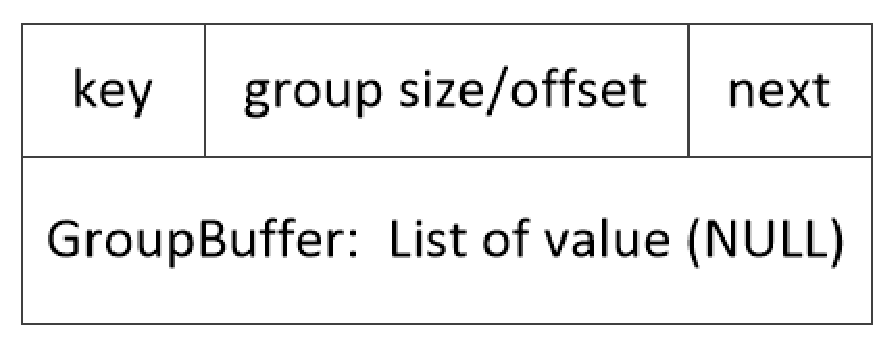
\includegraphics[width=.3\textwidth]{fig/EntryStructure}
\caption{the Entry Structure of the Group Size Accumulating Hash Table.}
\end{figure}
We buffer the partial grouping result in the entry of the hash table. During group size accumulating algorithm runs, the GroupBuffer filed is NULL in case of costing memory. With kv-pairs to be aggregated coming, values will be buffered in the entry that they belong to at first. The size of buffer used is the sum of the size of each GroupBuffer. If the size of buffer used achieves the maximum threshold, traverse the hash buckets contained by the sub file being processed and the partial grouping data will be output to the result file sequentially. Recall to 3.2 section, we convert the group size to the initial offset of a group. The offset of the current group ${off}_{cur}$ equals to the sum of ${off}_{pre}$ (the offset of the previous group) and  $f_{pre}$( the size of data contained by the previous group), which means that the stored location of the previous group must be prior to the current group. Thus, the seek operation for the current entry can base on the previous seek operation, i.e., the seek operations of all kv-pairs follow a top to down pattern in the result file. In this way, seek operations of different groups will be in order, it allows us to flush the buffer by scanning sequentially the result sub file. Note that, even though a random seek is performed, the seek time is expected to be very small because the next offset is physically very close to the current disk head position. The experiment shows that the gain is up to 10\%.
\end{comment}

%\subsection{Cost Analysis}

%Let $F$ be the input file, $n=|F|$ be the number of records, $G$ be the number of groups, $LB$ be the longest bucket in the hash table and $L$ be the largest linked list that stores the offset of each occurrence of a group for the bucket. In the worst case, $|LB|=O(n)$  and $|L|=O(n)$ . To see this, consider the input file $F$ for which $n=|F|$, each $\langle groupkey,valuesize\rangle$ are inserted to a hash bucket in group size accumulating phase, the worst complexity is $|L|$. The overall worst case complexity of group size accumulating is $n\cdot|L|$. For the hash grouping phase, each offset of a kv-pair needs to search the hash table, the query time is  $|L|$ in the worst case. The overall worst case complexity is also $n\cdot|L|$. Therefore, the overall worst case complexity of bHash is $2n \cdot|L|$ which is $O(n^2)$ time. However, in practice and in all application scenarios  $L \ll n$ and  $LB \ll n$ hold. The worst case above has supposed that is equal to $n$, e.g., each record is a group and all kv-pairs are mapped to a bucket. In fact, it is unusual because the target of the Hash technology is to uniform hash. The time to query and insert the hash table is almost constant order of magnitude so it is reasonable to expect that $L$ and $B$ are orders of magnitude far smaller than $n$. Thus, the overall expected complexity bound of bHash is much better than the worst case bound. This is also verified by the experimental evaluation, which demonstrated that bHash scales almost linearly to $n$.


